\chapter{Interaktion per GUI}
\chplbl{bed-gui}
Im zweiten Teil der Aufgabe sollte eine \gls{gui} für den \md entwickelt werden -- die \mdg. Wie wird diese bedient? Worauf ist zu achten? Was unterscheidet sich die \mdg vom \md? Diese Fragen möchte ich in diesem Kapitel beantworten.%Am Ende des Kapitels biete ich wie für den \md ein Tutorial an, welches Dir die Funktionsweise der \mdg an einem Beispiel nahebringen soll.

Auch die \mdg erfordert keine Installation -- die \mdg ist nach dem Entpacken der \datei{zip} unmittelbar ausführbar. Die Schritte vom Herunterladen bis zum Starten der \mdg sind dabei analog zum \md:

\begin{enumerate}
\item Die Datei \texttt{micro-debug-gui-version.zip} von der Projektseite \cite{Roesch2012gui} herunterladen
\item Die \datei{zip} in ein beliebiges Verzeichnis entpacken (bspw. \texttt{/opt/micro-debug-gui/})
\item Das Verzeichnis der \mdg dem \texttt{PATH} hinzufügen
\item Die \mdg starten -- mit \texttt{micro-debug-gui.sh~-{}-help}
\end{enumerate}

Die \mdg ist technisch eine eigenständige Anwendung, die den \md benutzt -- wie ich in \chpref{gui} erläutere. Der Code des \md ist daher in der \mdg enthalten und kann mit wenigen Anpassungen ohne \gls{gui} benutzt werden. Dies möchte ich nun kurz genauer erklären.

\section{Nutzung der Konsolenvariante}
\seclbl{gui-nutzung-konsole}
Nach dem Entpacken der \datei{zip} entsteht eine ähnliche Verzeichnis-Struktur, wie beim \md. Allerdings existiert nun das Verzeichnis \texttt{lib/}, das unter anderem eine \datei{jar} beinhaltet, die den Code des \md enthält -- die Datei \texttt{micro-debug-version.jar}.

Ich möchte nun zeigen, wie man die \mdg so ergänzt, dass sowohl die \mdg als auch der \md aufrufbar sind. Da dieses Verhalten für Windows und Linux analog ist, zeige ich es am Beispiel von Linux. \lstref{parallele-nutzung-md-mdg} enthält die Kommandos, die für diese Ergänzung auf der Konsole nötig sind.

\begin{lstlisting}[language=sh,caption={Parallele Nutzung des \md und der \mdg},label=\lstlbl{parallele-nutzung-md-mdg}]
cd micro-debug-gui-version/
cp micro-debug-gui.sh micro-debug.sh
\end{lstlisting}

Als Basis für die parallele Nutzung kann das Startskript der \mdg kopiert werden; diese Kopie (\texttt{micro-debug.sh}) musst aber noch angepasst werden:
\begin{enumerate}
\item Der Text \texttt{"\$DIR/micro-debug-gui-versiong.jar":"\$DIR/lib/*"} muss durch \texttt{"\$DIR/lib/micro-debug-versionk.jar"} ersetzt werden -- \emph{versiong} ist dabei die Version der \mdg und \emph{versionk} die Version des \md.

Hierdurch wird die Bibliothek geändert, die den auszuführenden Programmcode enthält.

\item Auch die Startklasse \texttt{com.github.croesch.micro_debug.gui.MicroDebug} muss durch \texttt{com.github.croesch.micro_debug.MicroDebug} ersetzt werden.
\end{enumerate}

Nach diesen Schritten sind zwei Startskripte vorhanden: Eines zum Start der \mdg und eines zum Start des \md. Beide können nun unabhängig voneinander ausgeführt werden.

\section{Unterschiede zur Konsolenvariante}
Die Struktur der \mdg ist ähnlich zur Struktur des \md, aber nicht identisch. Auch beim Aufruf und bei der Bedienung gibt es einige nennenswerte Unterschiede, die ich nun aufzeigen möchte.

\subsection{Parameter}
\seclbl{unterschied-parameter}
Bereits der Aufruf der \mdg unterscheidet sich von dem des \md: Es gibt weniger Parameter und die \mdg kann auch ohne Parameter aufgerufen werden. Alle der im Folgenden aufgeführten Parameter sind optional.

\begin{description}
\item[-h, -{}-help]
  mit diesem Parameter kann, wie beim \md, die Hilfe angezeigt werden lassen, die neben den verschiedenen Aufrufmöglichkeiten die möglichen Parameter erklärt. Zusätzlich werden auch hier noch einige ergänzende Informationen angezeigt.

\item[-v, -{}-version]
  gibt die Version der \mdg und des benutzten \md aus.
\end{description}

Wie der \md startet auch die \mdg nicht, wenn die Hilfe oder Version angezeigt werden soll, sondern beendet sich nach Ausgabe der Informationen.

Anders als der \md benötigt die \mdg die Pfade zu den Bytecode-Dateien nicht; diese werden direkt zu Beginn über die \gls{gui} eingegeben. Dies erkläre ich nochmal genauer im \secref{startfenster}.

\subsection{Verfügbare Funktionen}
Die \mdg benutzt den \md und hat daher prinzipiell Zugriff auf alle Funktionen, die der \md dem Benutzer bereitstellt. Da die \mdg dem Benutzer aber fortlaufend die Werte der Register und des Hauptspeichers, den \ma sowie den \ac anzeigt, ist es nicht nötig diese Werte beobachten zu können. Befehle wie \texttt{trace-reg} sind daher in der \mdg nicht wiederzufinden. Auch die Ausgabe des Stacks gibt es nicht mehr, denn dieser kann im Hauptspeicher angesehen werden.

Die Breakpoints werden dem Benutzer fortlaufend angezeigt und können über Mausklicks aktiviert und deaktiviert werden, daher fallen Befehle wie \texttt{ls-break} auch weg.

Die \mdg bietet demzufolge konstruktionsbedingt manche Funktionen nicht explizit an. Es gibt aber auch manche Funktionen, die bisher noch nicht über die \mdg abgebildet sind, diese sind:
\begin{itemize}
\item Einen Breakpoint für einen bestimmten Wert eines Registers zu setzen, wie beispielsweise per \texttt{break~Register~Wert}.
\item eine gewisse Anzahl an (Mikro-)Instruktionen auszuführen, wie per \texttt{micro-step~Zahl}.
\item den Wert eines Registers zu verändern, wie per \texttt{set~Register~Zahl}.
\item den Wert eines Wortes im Hauptspeicher zu setzen, wie per \texttt{set-mem~Zahl1~Zahl2}.
\end{itemize}

Diese Funktionen habe ich bisher aus Zeitgründen noch nicht implementiert, werde ich aber nach und nach ergänzen.

Allerdings bietet die \mdg dem Benutzer im Gegensatz zum \md die Möglichkeit, die laufende \mic zu unterbrechen. Wie ich in \secref{verarbeitung-benutzeraktionen-threads} erkläre, nutzt die \mdg zur Ausführung der \mic einen eigenen \emph{Thread}. Über die \gls{gui} kann dieser Thread dann mit Hilfe des \gls{edt} unterbrochen werden -- prinzipiell ist diese Funktion wie ein unbedingter Breakpoint.

\subsection{Geschwindigkeit}
Die \mdg nutzt die Funktionen des \md, um die \mic simulieren und debuggen zu können. Folglich kann die \mdg prinzipiell nicht schneller sein als der \md, sondern eher langsamer.

Diese Vermutung bestätigte sich bei ersten Tests der \mdg. Bei einfachen Befehlen, wie eine (Mikro-)Instruktion auszuführen oder die \mic zu resetten war kein Geschwindigkeitsunterschied beobachtbar. Aber besonders bei dem \texttt{run}-Befehl war deutlich zu beobachten, dass die \mdg mehr Zeit benötigte.

Was machte die \mdg besonders langsam? Wie konnte dieses Problem gelöst werden? Die Ursache der langsamen Ausführung war die Aktualisierung der \gls{gui}: Die Werte der Register und des sichtbaren Hauptspeichers, sowie die aktuell ausgeführte Zeile wurden ständig aktualisiert.

Ständig bedeutet, dass nach jedem Zyklus der \mic die \gls{gui} aktualisiert wurde. Ich habe daraufhin eine Konfigurationsoption -- \texttt{gui.update.after.each.tick} -- eingeführt; wird diese Option auf \texttt{true} gesetzt, aktualisiert die \mdg die \gls{gui} nach jedem Zyklus der \mic, eine deutlich längere Ausführungszeit kann beobachtet werden. Daher ist diese Option standardmäßig auf \texttt{false} gesetzt.

\section{Oberflächenelemente}
Nachdem ich nun einige Eigenschaften der \mdg beschrieben habe, möchte ich jetzt einen detaillierteren Einblick in die \mdg geben. Dazu werde ich die verschiedenen Hauptkomponenten der \mdg zeigen und deren Funktionen erklären.

\subsection{Startfenster}
\seclbl{startfenster}
Wie ich in \secref{unterschied-parameter} beschrieben habe, werden der \mdg die Pfade der Bytecode-Dateien nicht als Parameter übergeben -- es gibt ein extra Fenster dafür. Dieses Fenster erscheint unmittelbar nach dem Start der \mdg und ist in \figref{start-frame-empty} zu sehen.

\begin{figure}[h]
	\centering
	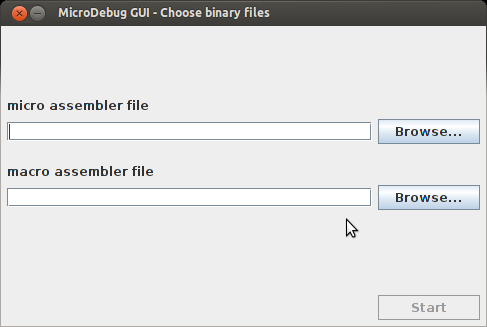
\includegraphics[width=6cm]{images/start-frame-empty}
	\caption{Screenshot des Start-Fensters}
	\figlbl{start-frame-empty}
\end{figure}

Wenn zwei Pfade eingegeben sind, kann die \mic dann über den Start-Button initialisiert werden und die \mdg ist funktionsbereit. Bei der Initialisierung der \mic werden die beiden Bytecode-Dateien auf ihre Gültigkeit geprüft; zuerst die Mikro-Assembler-Datei und dann die Assembler-Datei. Falls eine der Dateien ungültig ist, wird statt dem Hauptfenster der \mdg erneut das Start-Fenster gezeigt. In diesem Fall ist dann das Textfeld mit der ungültigen Datei leer, wie beispielsweise in \figref{start-frame-both-wrong} zu sehen.

\begin{figure}[h]
	\centering
	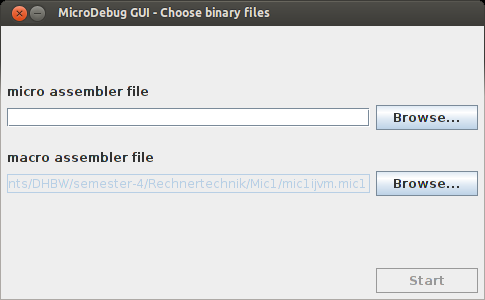
\includegraphics[width=6cm]{images/start-frame-both-wrong}
	\caption{Screenshot des Start-Fensters -- die angegebenen Dateien waren \emph{beide} ungültig}
	\figlbl{start-frame-both-wrong}
\end{figure}

In diesem Beispiel waren beide Dateien ungültig, aber nur ein Textfeld ist leer. Warum? Die \mdg prüft die Dateien nacheinander, ist die erste Datei bereits ungültig, wird die zweite nicht geprüft und zunächst als gültig angenommen. Das Textfeld der zweiten Datei ist dann inaktiv, kann aber mit einem Doppelklick wieder aktiviert und dadurch editiert werden. In dem genannten Beispiel habe ich das getan und anschließend zwei korrekte Dateien eingetragen, wie in \figref{start-frame-both-filled} abgebildet ist.

\begin{figure}[h]
	\centering
	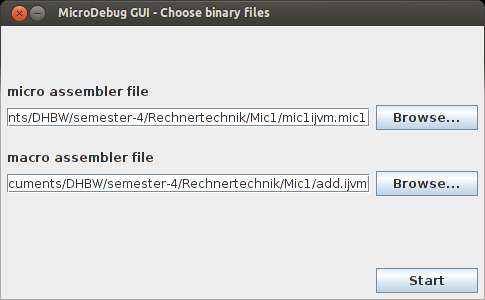
\includegraphics[width=6cm]{images/start-frame-both-filled}
	\caption{Screenshot des Start-Fensters mit zwei eingetragenen Dateien}
	\figlbl{start-frame-both-filled}
\end{figure}

Wurden zwei gültige Dateien eingetragen, startet die \mdg und öffnet das Hauptfenster aus \figref{main-frame-onbegin}.

\begin{figure}[h]
	\centering
	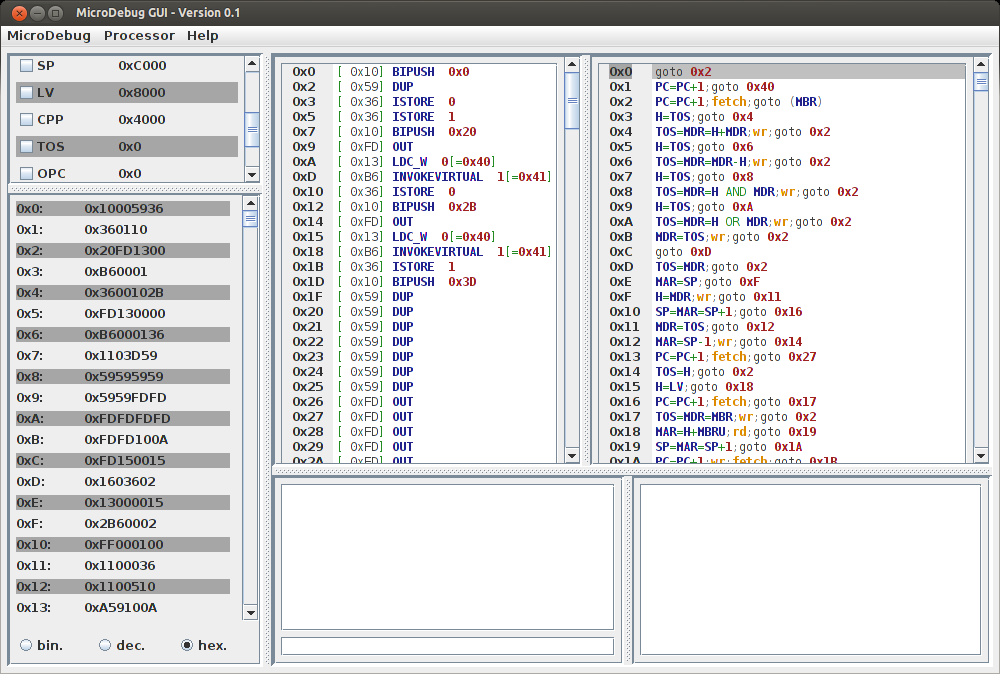
\includegraphics[width=0.8\linewidth]{images/main-frame-onbegin}
	\caption{Hauptfenster der \mdg zu Beginn}
	\figlbl{main-frame-onbegin}
\end{figure}

\subsection{Register}
In \figref{main-frame-onbegin} sind links oben die Register mit ihren Werten zu sehen; die gleiche Ansicht ist in \figref{main-frame-registers} nochmal größer dargestellt.

\begin{figure}[h]
	\centering
	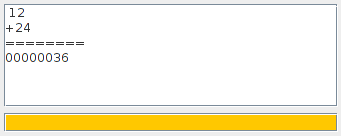
\includegraphics[width=4cm]{images/main-frame-mic-ta}
	\caption{Textkomponenten zur Ein- und Ausgabe der \mic im Hauptfenster der \mdg}
	\figlbl{main-frame-mic-ta}
\end{figure}

\begin{figure}[h]
	\centering
	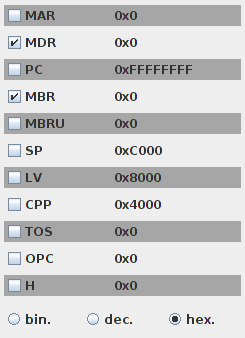
\includegraphics[width=4cm]{images/main-frame-registers}
	\caption{Registeransicht im Hauptfenster der \mdg}
	\figlbl{main-frame-registers}
\end{figure}

Die Checkboxen repräsentieren die Breakpoints für die Register, in \figref{main-frame-registers} hält die \mic demnach an, wenn \reg{MBR} oder \reg{MDR} im nächsten Zyklus geschrieben wird. Über die Radiobuttons unten kann das Zahlenformat der Registerwerte geändert werden: auf binär, dezimal oder hexadezimal. So kann der Benutzer für jeden Zweck die optimale Darstellung der Registerwerte wählen.

\subsection{Hauptspeicher}
Unter der Registeransicht befindet sich im Hauptfenster die Ansicht des Hauptspeichers. Hier kann wie bei der Registeransicht das Zahlenformat der Hauptspeicherwerte jederzeit geändert werden.

In der Ansicht des Hauptspeichers sind nur eine feste Anzahl an Einträgen zu sehen, die sich nicht dynamisch an die Größe des sichtbaren Bereichs anpassen. Dies habe ich wegen der besseren Performanz so gelöst.

Die Ansicht zeigt den gesamten Hauptspeicher -- neben den lokalen Variablen, dem Stack und den Konstanten kann dadurch auch der disassemblierten \ac in Bit-Form betrachtet werden.

\subsection{Text-Ein- und -Ausgabe}
Rechts neben der Hauptspeicheransicht sind im Hauptfenster unten verschiedene Textkomponenten zu sehen. Deren Funktion sollte spätestens im laufenden Betrieb der \mdg deutlich werden: Links unten ist die Textkomponente, um der \mic Text bereitzustellen. Darüber befindet sich die Textkomponente, die die Ausgaben der \mic anzeigt und im rechten Bereich ist die Textkomponente, die Informationen des \md anzeigt, die sonst auf der Konsole ausgegeben würden und bisher noch keinen Platz in der Oberfläche bekommen haben.

\figref{main-frame-mic-ta} zeigt, wie sich das Eingabefeld für die \mic verhält, wenn die \mic per \texttt{IN} ein Zeichen liest, aber der Puffer des \md keine Zeichen mehr enthält: es wird orange gefärbt. In diesem Fall sollte der nächste Text für die \mic eingegeben und mit \emph{ENTER} bestätigt werden. Dadurch werden die eingegebenen Zeichen inklusive Zeilenumbruch im \md gepuffert, bis sie die \mic einliest.

Es können durch diese Textkomponente auch Eingaben gemacht werden, wenn der Puffer des \md noch nicht leer ist. In diesem Fall wird der Text, der eingegeben wird, dem Puffer des \md angehängt. So können schon zu Beginn alle nötigen Texteingaben gemacht werden und anschließend der \ac ohne Unterbrechung ausgeführt werden.

\subsection{Code}
Die wohl wichtigsten zwei Komponenten befinden sich in \figref{main-frame-onbegin} rechts oben: Der disassemblierte \ma und \ac. Die beiden Ansichten sind von der Funktion identisch aufgebaut und zeigen den disassemblierten Code mit Syntaxhervorhebung, Zeilennummern und den dazugehörigen Breakpoints an. Zusätzlich wird die Zeile des Codes hervorgehoben, die als nächstes ausgeführt wird.

\begin{figure}[h]
	\centering
	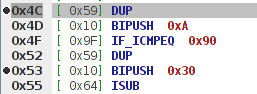
\includegraphics[width=4cm]{images/main-frame-code-part}
	\caption{Ausschnitt des \ac im Hauptfenster der \mdg}
	\figlbl{main-frame-code-part}
\end{figure}

\figref{main-frame-code-part} zeigt einen Ausschnitt der Code-Ansicht. Hier ist zu sehen, dass als nächstes die Zeile \texttt{0x4C} abgearbeitet werden wird und dass in den Zeilen \texttt{0x4C} und \texttt{0x53} Breakpoints gesetzt sind. Die Breakpoints werden durch einen Doppelklick gesetzt und durch einen Doppelklick können sie wieder entfernt werden. Der Doppelklick muss an der Stelle ausgeführt werden, an der die Breakpoints gezeichnet werden -- links neben den Zeilennummern.


%\section{Tutorial}